\chapter{Mediciones con el sistema}
Se realizaron mediciones con los diferentes espectrómetros para compararlos con nuestro sistema. El espectro de la lámpara de mercurio fue medido con el espectrómetro HR4000 con dos tiempos de integración diferentes. Se observa la medición con 8ms de tiempo de integración en la figura \ref{fig:hr40004ms}(a) y con 100ms de integración \ref{fig:hr40004ms}(b). Se aprecia como el sistema se satura en varias de las líneas de emisión.
\begin{figure}[h]
	\centering
	\subfigure[HR4000, tiempo de integración 8ms]{	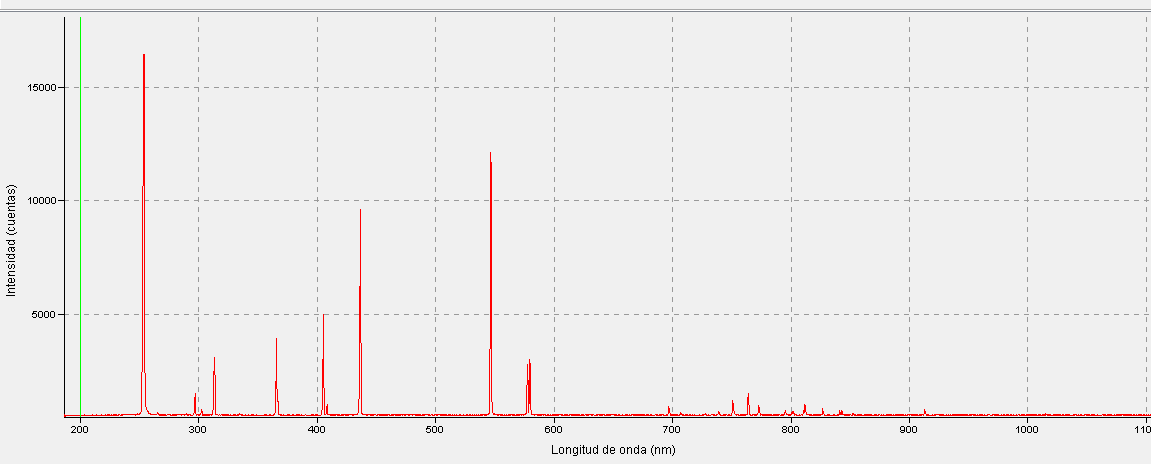
\includegraphics[width=0.9\linewidth, height=5cm]{Imagenes/4/HR4000_4ms}}
	%\subfigure[HR4000 40ms]{	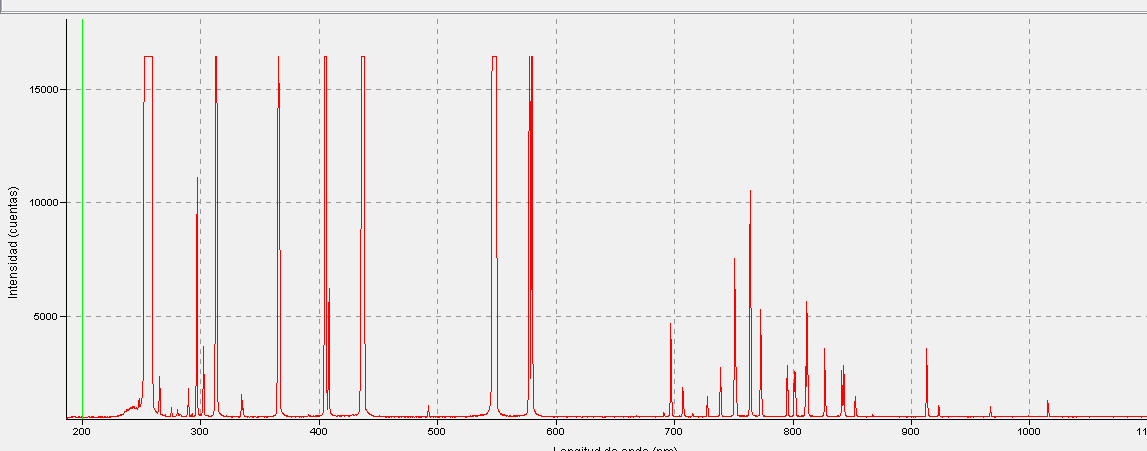
\includegraphics[width=0.6\linewidth]{Imagenes/4/HR4000_40ms}}
	\subfigure[HR4000, tiempo de integración 100ms]{	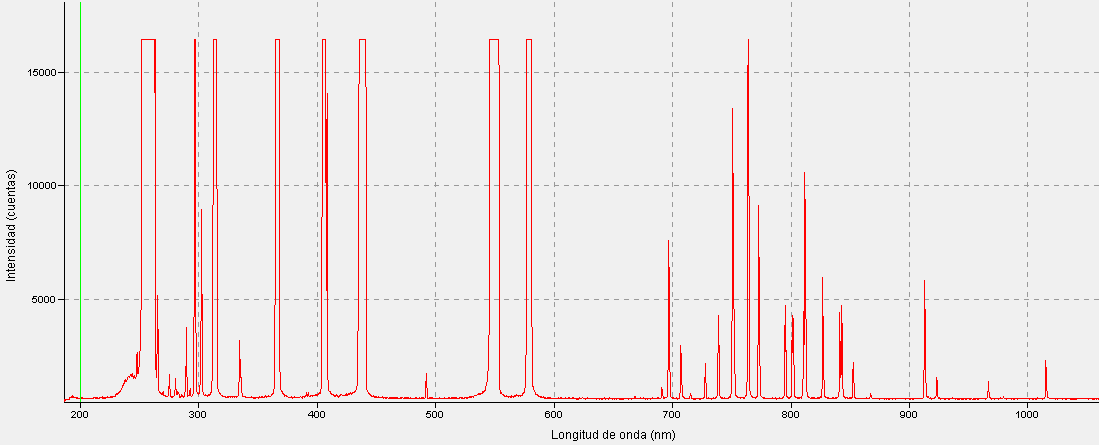
\includegraphics[width=0.9\linewidth, height=5cm]{Imagenes/4/HR4000_100ms}}
	\caption{Espectro de la lámpara de mercurio medido con el espectrómetro HR4000. Se utilizan dos tiempos de integración diferentes.}
	\label{fig:hr40004ms}
\end{figure}
% figura 1
\\
Se tiene el espectro de la lámpara de mercurio medido con el espectrómetro QE65000, el cual a los 8ms de tiempo de integración (el cual es el valor mínimo que acepta), se visualiza como se satura en ciertas longitudes de onda, ver figura \ref{fig:qe650008mshg}.
\begin{figure}[h!]
	\centering
	\subfigure[Espectro de la lámpara de mercurio con un tiempo de integración de 8ms, mínimo del sistema.]{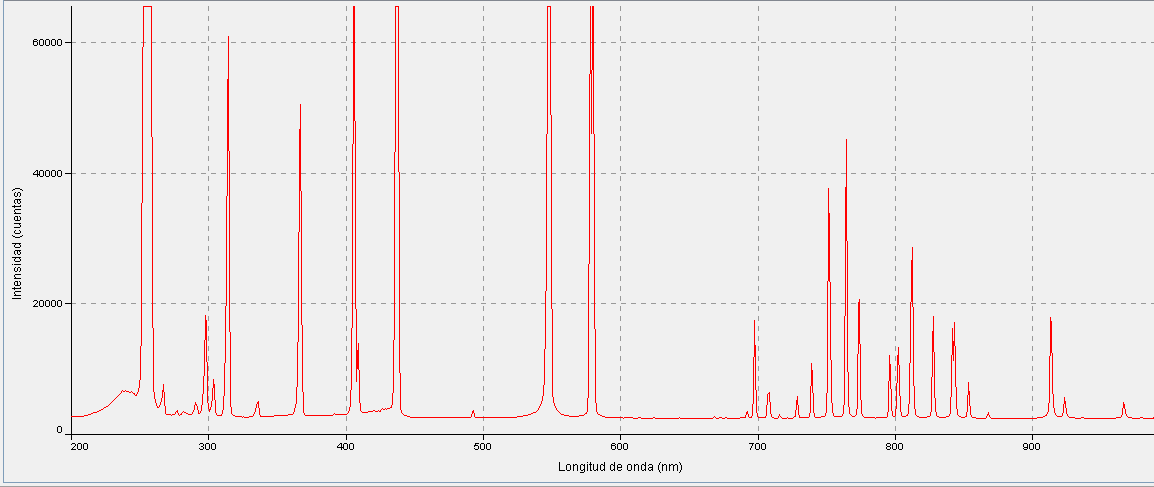
\includegraphics[width=0.9\linewidth, height=4.5cm]{Imagenes/4/QE65000_8msHg}}
	%\subfigure[QE65000 40ms]{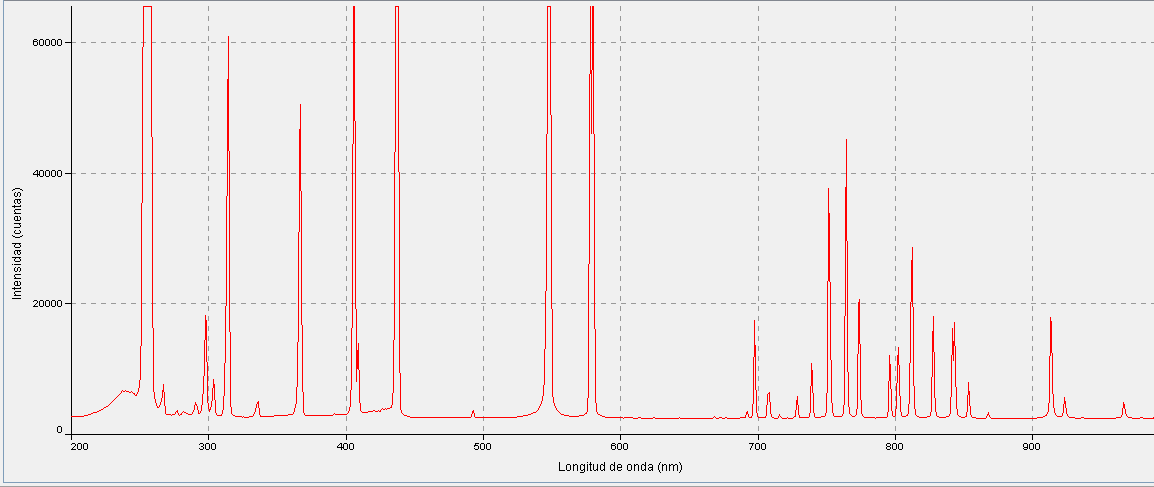
\includegraphics[width=0.6\linewidth]{Imagenes/4/QE65000_8msHg}}
	\subfigure[Espectro de la lámpara de mercurio con un tiempo de integración de 100 ms.]{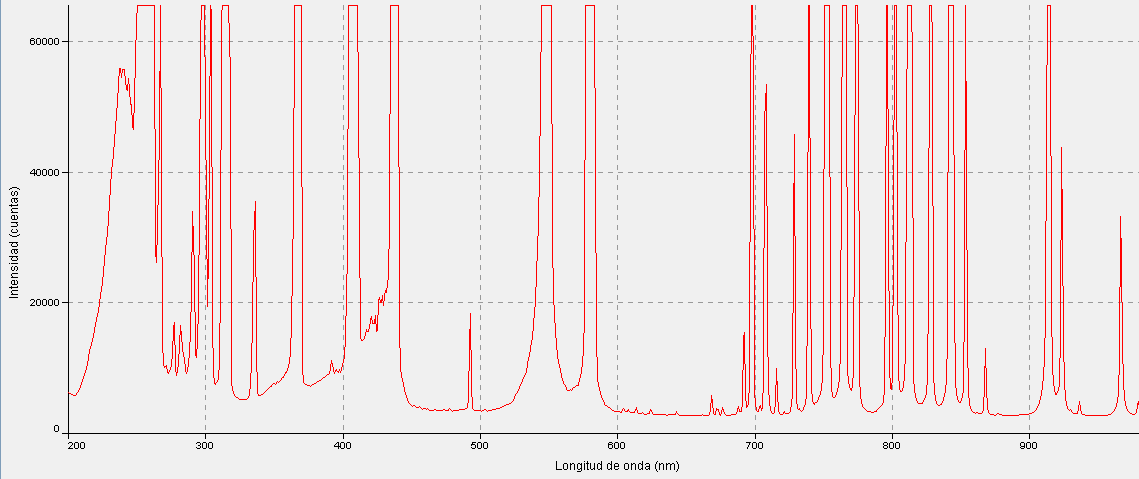
\includegraphics[width=0.9\linewidth, height=4.5cm]{Imagenes/4/QE65000_100msHg}}
	\caption{Espectro de la lámpara de mercurio adquirido con el espectrómetro QE65000. Se aprecia cómo se satura en una gran cantidad de  líneas.}
	\label{fig:qe650008mshg}
\end{figure}
%figura 2

Con el sistema propuesto todas las mediciones se hacen con los \textit{slits} de entrada y de salida en 10$\mu$m, para tener la mayor resolución.  En la figura \ref{fig:spectra100}, se está usando el máximo de sensibilidad en el PMT.
\begin{figure}[h!]
	\centering
	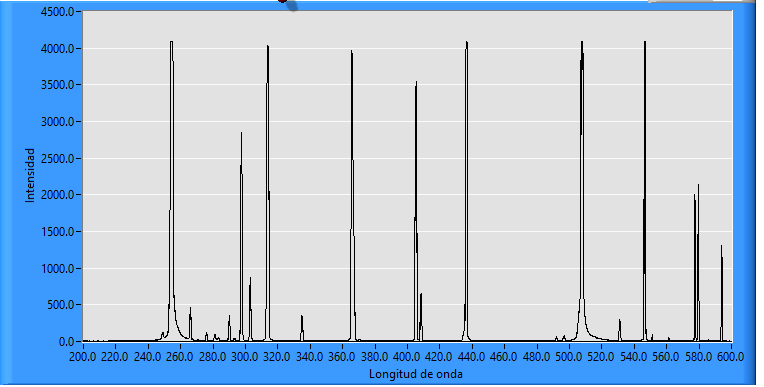
\includegraphics[width=0.9\linewidth, height=5cm]{Imagenes/4/spectra100}
	\caption{Espectro de la lámpara de mercurio medido con el sistema desarrollado. El monocromador tiene los \textit{slits} de entrada y salida en su menor apertura, 10$\mu$m, y en el máximo de sensibilidad del \textbf{PMT}.}
	\label{fig:spectra100}
\end{figure}
%figura 3
%\newpage
Dentro de las 12 líneas de emisión del espectro de mercurio, que se usaron para calibrar. Hay dos que se encuentran relativamente cerca. las líneas tienen la longitud de onda de 576.96 nm y 579.066 nm. En la figura \ref{fig:lineasdos}(a) se observa como el QE65000 apenas logra distinguir las dos líneas, el HR4000, figura \ref{fig:lineasdos}(b) las resuelve sin problemas. Mientras que el sistema desarrollado logra resolver con mayor facilidad estas mismas líneas, véase figura \ref{fig:lineasdos}(c). 

\begin{figure}[h]
	\centering
	\subfigure[Líneas de emisión medidas con el QE65000, tiempo de integración 8ms.]{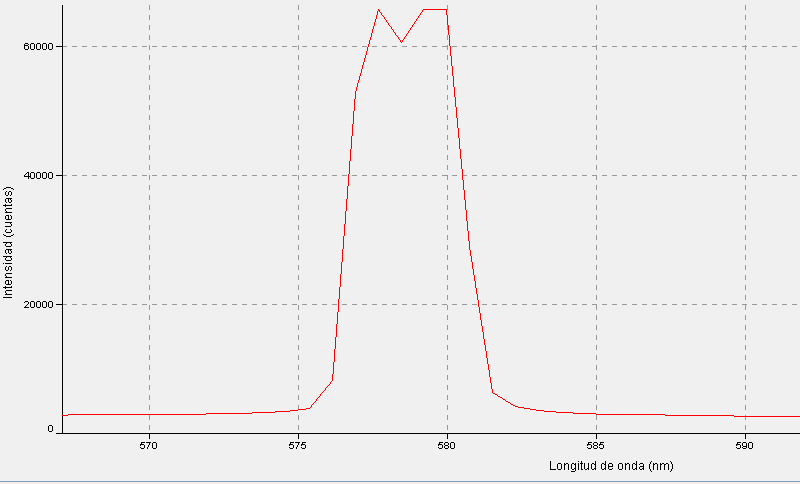
\includegraphics[width=0.48 \linewidth,height=3cm]{Imagenes/4/picosqe}}
	\subfigure[Líneas de emisión medidas con el HR4000, tiempo de integración 3.8ms]{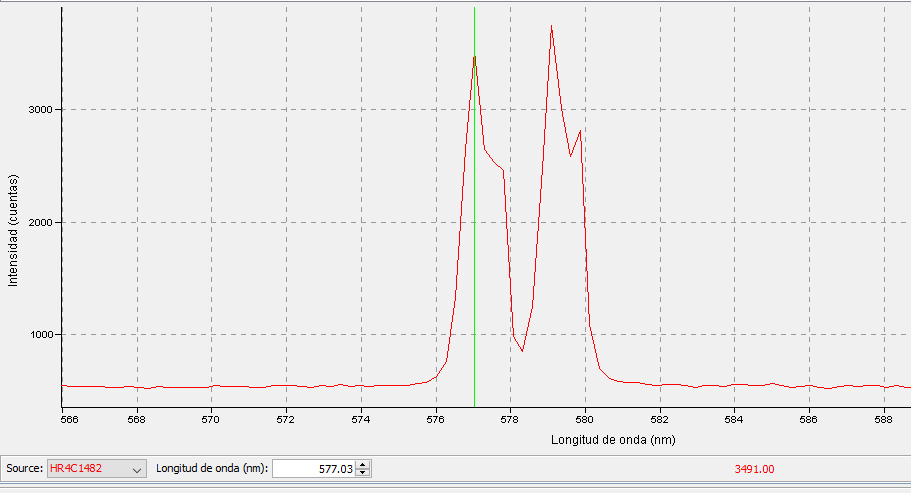
\includegraphics[width=0.48\linewidth,height=3cm]{Imagenes/4/picoshr}}
	\subfigure[Líneas de emisión medidas con el sistema desarrollado. Slits de entrada y salida a 10$mu$m, sensibilidad 0.8v.]{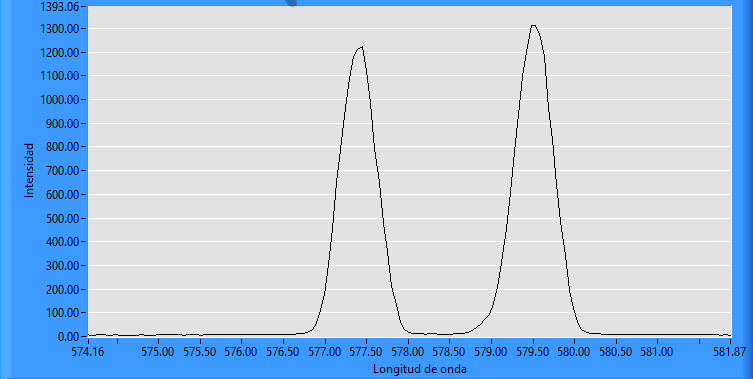
\includegraphics[width=0.8\linewidth,height=4.5cm]{Imagenes/4/picos}}
	\caption{Dos de las líneas de emisión de la lámpara de mercurio $\lambda$= 576.96nm y 579.066 nm. Se aprecia que el sistema desarrollado resuelve mejor estas dos líneas de emisión.}
	\label{fig:lineasdos}
\end{figure}
%\begin{figure}[h]
%	\centering
%	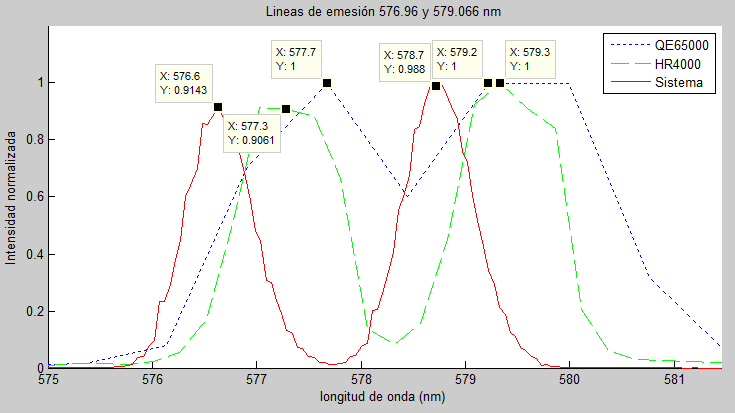
\includegraphics[width=10cm, height=5cm]{Imagenes/4/picosT}
%	\caption[líneas de emisión de la lámpara de mercurio, (576.96nm y 579.066nm)]{líneas de emisión de la lámpara de mercurio, (576.96nm y 579.066nm), se observan pequeñas diferencias entre los sistemas.}
%	\label{fig:picost}
%\end{figure}

%figura 4

En la figura \ref{fig:lst} se visualizan el espectro de la lámpara de tungsteno-halógeno medido con los espectrómetros QE65000, HR4000 y el sistema desarrollado. Como se puede apreciar los espectros con que se cuentan tienen un intervalo de medición mayor al del sistema desarrollado. 
El sistema desarrollado puede medir hasta los 780nm, donde el valor máximo de lectura está en los 544.6 nm. A partir de los 600nm comienza a decaer de forma rápida su sensibilidad. Aún y cuando  el intervalo que el sistema puede medir es menor tiene mejor resolución que los espectrómetros, HR4000 y QE65000 como se ve en la figura \ref{fig:lineasdos}.

\begin{figure}[h]
	\centering
	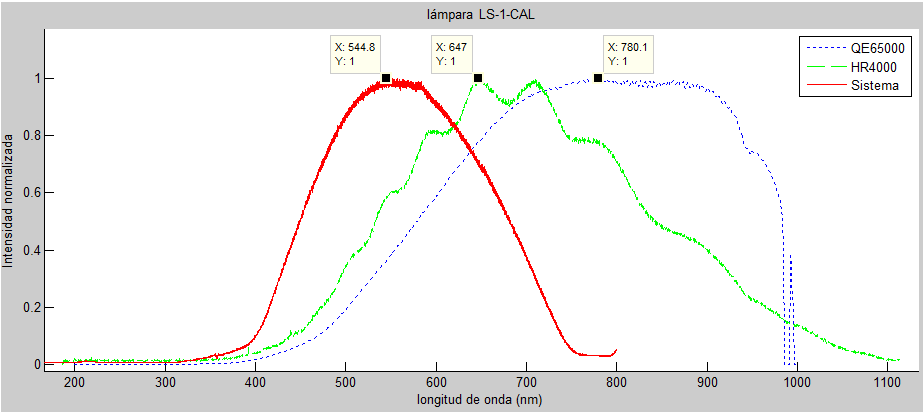
\includegraphics[width=0.9\linewidth,height=4.5cm]{Imagenes/4/ls_t}
	\caption[Espectro de la lámpara LS-1-CAL]{Lámpara LS-1-CAL, medida con los espectrómetros, HR4000 (verde) y QE65000 (azul), y el sistema desarrollado (rojo). Se observa que el sistema tiene un intervalo menor que el de los dos espectrómetros.}
	\label{fig:lst}
\end{figure}

Se midieron diferentes fuentes luminosas. Donde se encuentran pequeñas diferencias entre los espectrómetros. En la figura \ref{fig:uv380t} se visualiza el espectro de un LED ultravioleta, y una diferencia de 2nm entre nuestro sistema y el QE65000. La figura \ref{fig:uv400} es el espectro de un LED violeta, 400nm, hay una gran similitud entre las tres mediciones(a). Con una diferencia de máximo 0.8nm entre los picos máximos (b). Un LED rojo $\lambda$ = 650nm, se obtienen resultados similares al LED violeta $\lambda$ = 400nm, véase figura \ref{fig:rojot}(a), donde la diferencia mayor es de 0.6nm ver figura \ref{fig:rojot}(b). En el LED rojo de 700nm encontramos ya una diferencia notoria de casi 20nm, ver figura \ref{fig:r700}, entre el sistema y los dos espectrómetros, 
\begin{figure}[h]
	\centering
	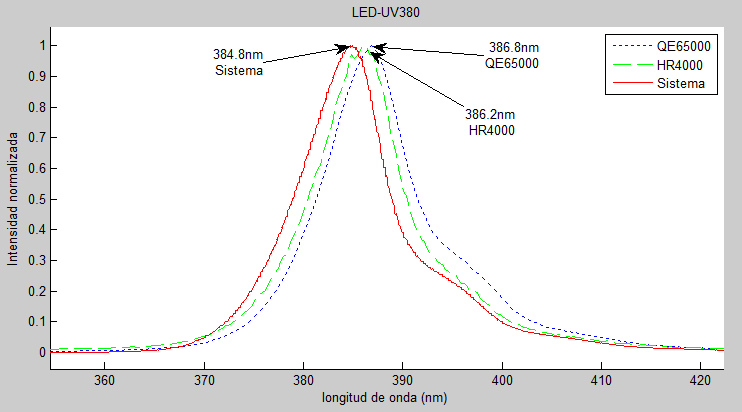
\includegraphics[width=0.9\linewidth,height=4.5cm]{Imagenes/4/uv380t}
	\caption[Espectro del LED Ultravioleta 380nm]{Espectro del LED Ultravioleta 380nm. Medido con los dos espectrómetros, (HR4000 y QE65000) y el sistema desarrollado. La gráfica se encuentra normalizada.}
	\label{fig:uv380t}
\end{figure}

\begin{figure}[h]
	\centering
	\subfigure[Espectro del LED violeta, 400nm]{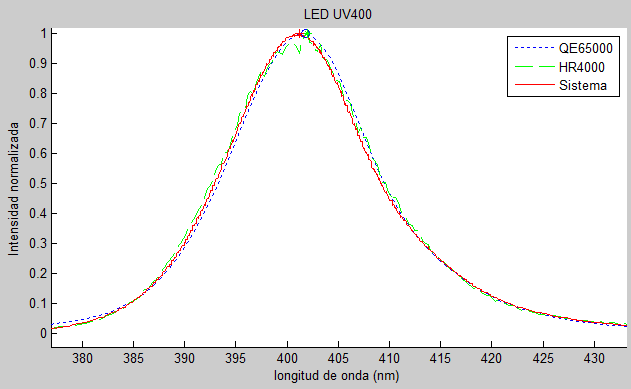
\includegraphics[width=0.48\linewidth, height=3.5cm]{Imagenes/4/UV400}}
	\subfigure[Acercamiento a los máximos.]{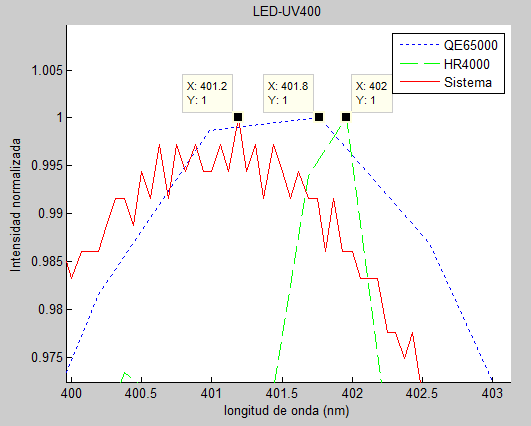
\includegraphics[width=0.48\linewidth,height=3.5cm]{Imagenes/4/UV400m}}
	
	\caption[LED violeta $\lambda$= 400nm]{LED violeta $\lambda$=400nm, medido con los espectrómetros HR4000(verde), QE65000(azul) y el sistema (rojo). Los tres instrumentos obtienen el mismo espectro(a). Las diferencias son tan pequeñas que solo se notan al acercarnos al espectro (b).}
	\label{fig:uv400}
\end{figure}
\begin{figure}[h]
	\centering
	\subfigure[LED rojo $\lambda$]{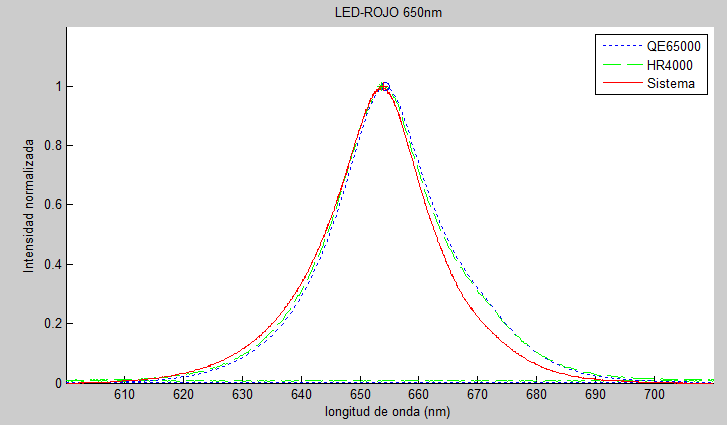
\includegraphics[width=0.48\linewidth, height=3.5cm]{Imagenes/4/rojot}}
	\subfigure[Acercamiento a los máximos]{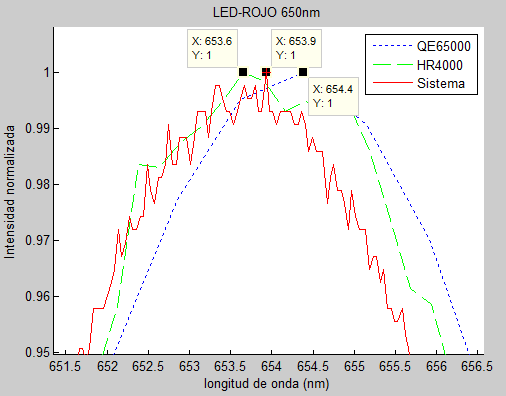
\includegraphics[width=0.48\linewidth, height=3.5cm]{Imagenes/4/rojom}}

	\caption[LED rojo $\lambda$ = 650nm]{LED rojo $\lambda$ = 650nm medido con los tres sistemas, al igual que con el LED UV $\lambda$= 400nm, se obtiene espectros muy similares (a). Acercándose se observan las pequeñas diferencias que hay en el pico de cada medición (b).}
	\label{fig:rojot}
\end{figure}
\begin{figure}[h]
	\centering
	\subfigure[Espectro del LED rojo $\lambda$=700nm]{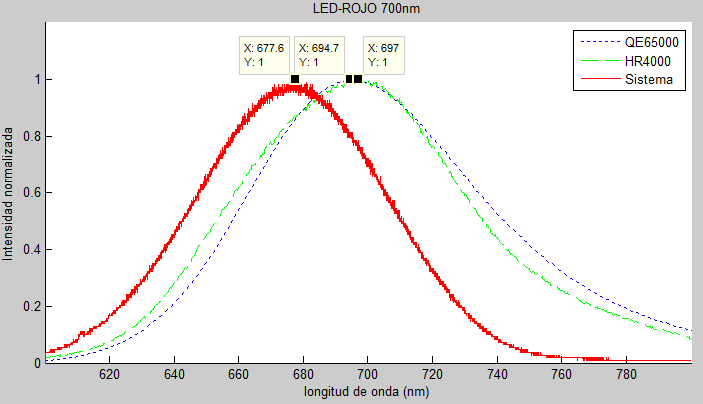
\includegraphics[width=0.8\linewidth,height=4cm]{Imagenes/4/r700}}
	\caption[LED rojo, de longitud de onda 700nm]{LED rojo ($\lambda$=700nm) medido con los tres sistemas. En este espectro es donde se observa una diferencia de casi 20nm entre el espectro medido con el sistema y los dos espectrómetros (HR4000 y QE65000).}
	\label{fig:r700}
\end{figure}
\clearpage
Al graficar el espectro del LED rojo ($\lambda$ = 700nm) sobre la respuesta de los sistemas ante la lámpara LS-1-CAL, vemos que el LED rojo está en una zona donde el sistema tiene una menor respuesta y que esta disminuye cada que avanza, figura \ref{fig:ls-rojo}. 

El error no se debe al ajuste que se realizó con \textbf{curve fitting tool}. En la gráfica que se observa en la figura \ref{fig:pasotam} podemos apreciar como al ir avanzando en la longitud de onda el paso es cada vez menor. Sin embargo, vemos que de los 650nm a los 700nm no hay una perdida que muestre que el pico del LED rojo en 700nm aparezca 20nm antes. Por ello concluimos que es por la sensibilidad del PMT y la eficiencia de la red, que el pico aparezca antes de lo esperado. 
\begin{figure}[h]
	\centering
	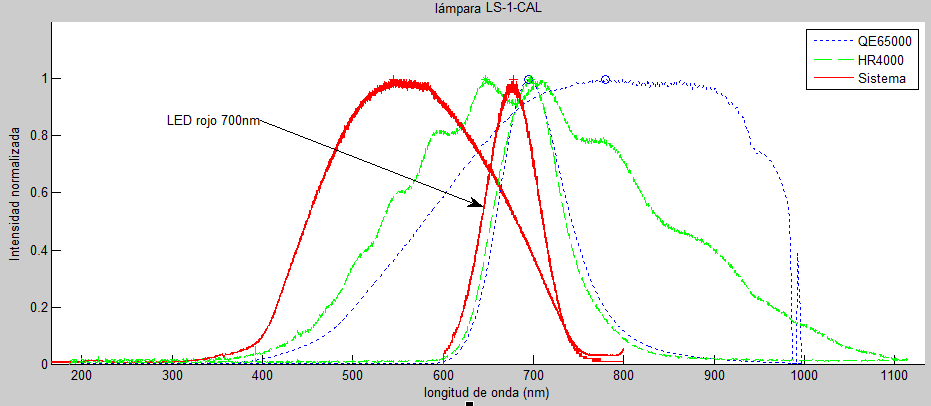
\includegraphics[width=0.9\linewidth,height=5cm]{Imagenes/4/ls-rojo}
	\caption{Espectro de la lámpara LS-1-CAL y el LED rojo $\lambda$ =700nm.}
	\label{fig:ls-rojo}
\end{figure}
\begin{figure}[h]
	\centering
	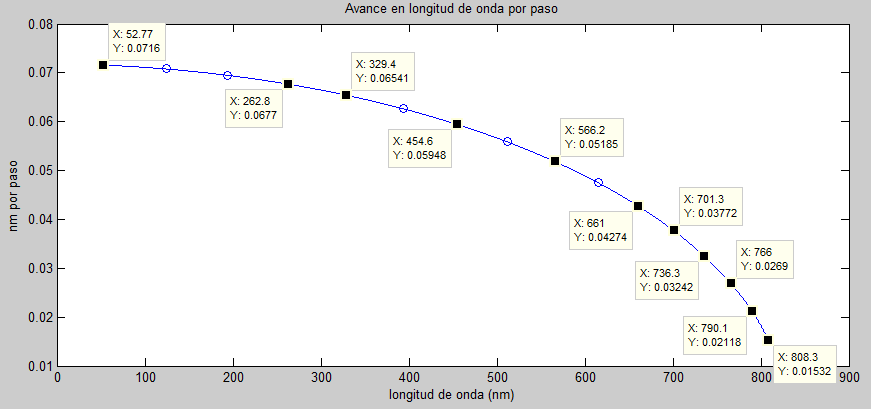
\includegraphics[width=0.9\linewidth,height=5cm]{Imagenes/4/pasotam}
	\caption{Longitud de onda que se avanza por paso.}
	\label{fig:pasotam}
\end{figure}

\newpage
\section{Ajuste en forma del espectro unidades relativas.}
La lámpara de LS-1-CAL tiene un intervalo desde los 300nm hasta más de los 1000nm. Como se observa en la figura \ref{fig:lst} el sistema desarrollado comienza a perder sensibilidad a partir de los 540nm. Así mismo se observa una medición incorrecta en el LED rojo de 700nm, ver figura \ref{fig:r700} el cual tiene un corrimiento de casi 20nm obteniendo el pico de emisión en 677.8 nm. 
En la tesis ''DISEÑO DE UN SISTEMA PORTÁTIL DE MEDICIÓN
DE IRRADIANCIA ESPECTRAL SOLAR
UTILIZANDO UN ESPECTRÓMETRO'' se realiza un ajuste de potencia de los espectrómetros QE65000 y HR4000 con la lámpara LS-1-CAL \cite{DeInvestigacion2020}. 

En la figura \ref{fig:ls-s-ds} se observa el espectro de la lámpara de tungsteno-halógeno. En azul es la medición con el sistema desarrollado y en rojo los valores de la lámpara con base en el ''\textit{datasheet}''.

\begin{figure}[h]
	\centering
	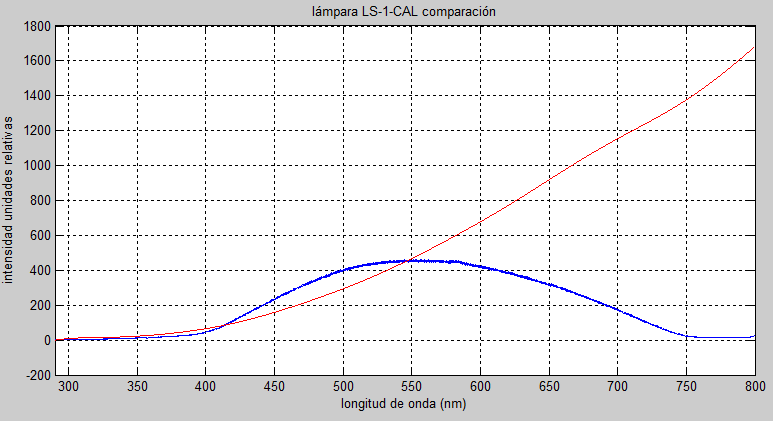
\includegraphics[width=0.9\linewidth]{Imagenes/4/LS-S-DS}
	\caption[Espectro de la lámpara LS-1-CAL, \textit{datasheet} (rojo), sistema (azul)]{Espectro de la lámpara LS-1-CAL, \textit{datasheet} (rojo), sistema (azul)}
	\label{fig:ls-s-ds}
\end{figure}

Al realizar diferentes mediciones con el sistema, variando la potencia, modificando la distancia de la lámpara LS-1-CAL, se obtuvieron las siguientes gráficas, ver figura \ref{fig:ls-potencia}. Donde en la figura \ref{fig:ls-potencia} (a) se tienen mediciones a diferentes potencias en unidades relativas. En la figura \ref{fig:ls-potencia} (b) se observan las mismas gráficas normalizadas. Se ve que el sistema tiene una linealidad en cuanto a la potencia. Con esta información se realiza un ajuste en forma del espectro.  

En la figura \ref{fig:ajusteenforma} se ve como el ajuste realizado hace coincidir el espectro medido con el del \textit{''datasheet''}. La medición del sistema sigue siendo en unidades relativas corrigiendo la forma del espectro. 

\begin{figure}[t]
	\centering
	\subfigure[Espectro de la lámpara LS-1-CAL en unidades relativas.]{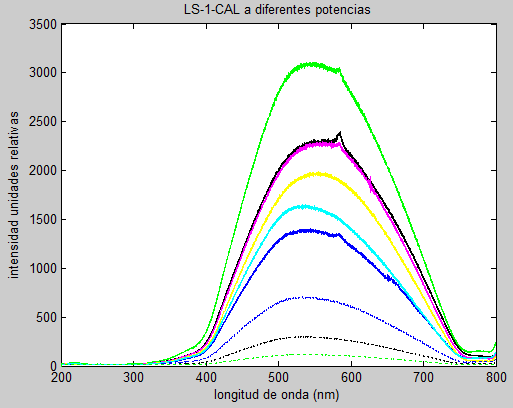
\includegraphics[width=0.4\linewidth, height = 3cm]{Imagenes/4/LS-potencia}}
	\subfigure[Espectro de lámpara LS-1-CAL normalizado.]{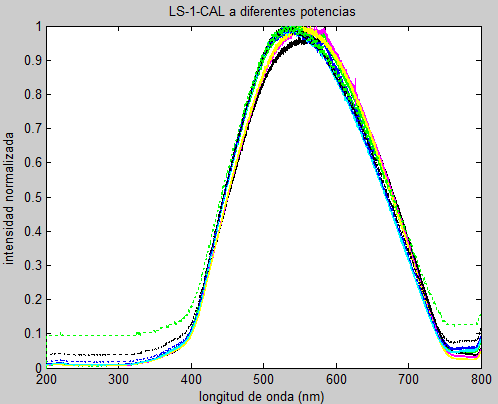
\includegraphics[width=0.4\linewidth,height = 3cm]{Imagenes/4/LS-potNor}}
	\caption{Espectro de la lámpara LS-1-CAL en unidades relativas.}
	\label{fig:ls-potencia}
\end{figure}

\begin{figure}[h]
	\centering
	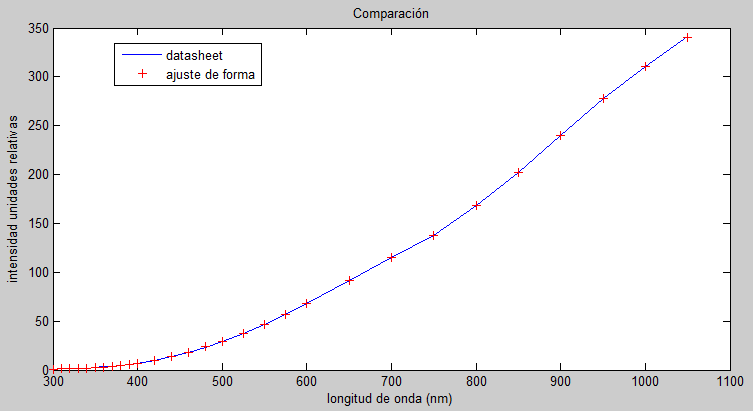
\includegraphics[width=0.8\linewidth]{Imagenes/4/ajusteEnForma}
	\caption[Espectro de la lámpara LS-1-CAL medido con el sistema con ajuste de forma]{Espectro de la lámpara LS-1-CAL medido con el sistema con ajuste de forma. En azul es el espectro obtenido en el datasheet, las cruces rojas son el espectro medido con el sistema desarrollado.}
	\label{fig:ajusteenforma}
\end{figure}

Al utilizar este ajuste de forma en la medición del LED rojo de 700nm se observa que su pico de emisión ya es correcto apareciendo a los 700nm, ver figura \ref{fig:ledrojoa}. Aún que a mayor longitud de onda se tiene que el ajuste ya no es optimo por la baja sensibilidad del sistema desarrollado. 
\begin{figure}[h]
	\centering
	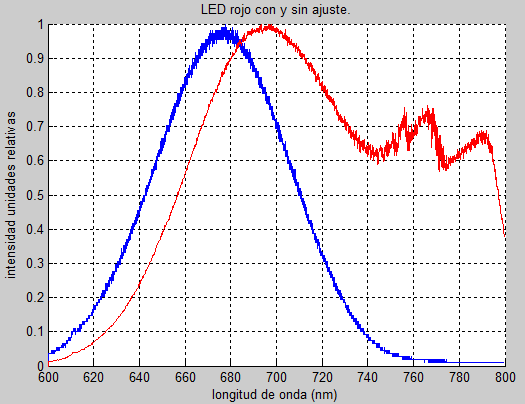
\includegraphics[width=0.8\linewidth,height=5cm]{Imagenes/4/LEDrojoA}
	\caption[Espectro de un LED rojo (700nm) con ajuste de forma.]{Espectro de un LED rojo (700nm) con ajuste de forma. Se observa que el pico del espectro con ajuste (rojo) ya tiene su pico de emisión a los 700nm a diferencia que sin ajuste (azul) esta en los 680nm aproximadamente.}
	\label{fig:ledrojoa}
\end{figure}

Dado que la lámpara LS-1-CAL tiene un intervalo de emisión de los 300nm en adelante. Este ajuste de forma solo nos sirve en un intervalo de 300nm a 700nm. El sistema desarrollado es capaz de detectar longitudes de onda menores a 300 nm por lo cuál se decide colocar la opción de utilizar o no este ajuste de forma. Al medir espectros de línea de emisión menores a 600nm no es necesario usar el ajuste. Al medir longitudes de ondas superiores a 300 nm se recomienda activar el ajuste de forma.



 
